\section{Experimental Analysis}
\label{sec:experimentdesign}

We performed a set of simulations to evaluate the performance of the heuristic algorithms and leverage the white space band influence on mesh network. 
The experiment set up is introduced in \ref{subsec:design} with the topology, metric calculation.
A set of result is shown in ~\ref{subsec:analysis} and analysis is presented with the throughput achieve through gateways.

\subsection{Experiment Design}
\label{subsec:design}

The capacity of a network binds with multiple factors, such as gateway placement, routing and also channel assignment. 
Stefano bring the good put in the network without considering the interference as maximum throughput to evaluate the channel assignment ~\cite{avallone2008channel}. 
However, without considering the interference, the traffic flow in the network is not scheduled.
And to find the best routing associate with channel assignment is out of our scope. 
Generally, an ISP will charge fee from customers according to the traffic achieve the gateways from wireless devices.
Our evaluation calculation targets on get the maximum throughput achieve the gateways.

In a mesh network, the bottleneck of the network are the links around the gateway nodes ~\cite{robinson2010deploying}. 
And any traffic transmitted to a wired gateway node is treated equally. So a methodology to get a scheduler maximum throughput is to serve the nodes close to the gateway nodes.
Thus to employ more capacity of the gateway neighbor links, the nodes close to the gateway nodes should be served first.
We first serve the nodes have 1 hop path to the gateway nodes, then choose the path has the least interference on the network and serve the demand as more as possible. Then we satisfy the demand of 2 hop layer nodes and so on, till there is no demand could be satisfied.
This calculation process is kind of routing protocol which help us to reach a scrollable maximum throughput of the network. For evaluation we keep the same calculation process for all the channel assignment algorithms. To find better solution for routing or capacity calculation is out of our scope.

% FIXME may need a validation of max calculation

\subsection{Analysis}
\label{subsec:analysis}
Most of the time clients of wireless network have different traffic demand. 
We first deploy a number of gateways according to number of mesh nodes randomly, 
   Then we randomly assign demand of mesh nodes with a max offer load,
   calculate the scalable maximum throughput, then repeat the process 20 times.
   The output is the average maximum throughput for this max offer load per mesh node.
   The performance of the two heuristic algorithms and ~\emph{CCA} ~\cite{draves2004routing}, ~\emph{BFSCA}  ~\cite{ramachandran2006interference} in a 30-node regular grid topology with 6MB link capacity in each channel are shown in figure ~\ref{fig:maxtpt}.

   \begin{figure}
   %\vspace{-0.0in}
   \centering
   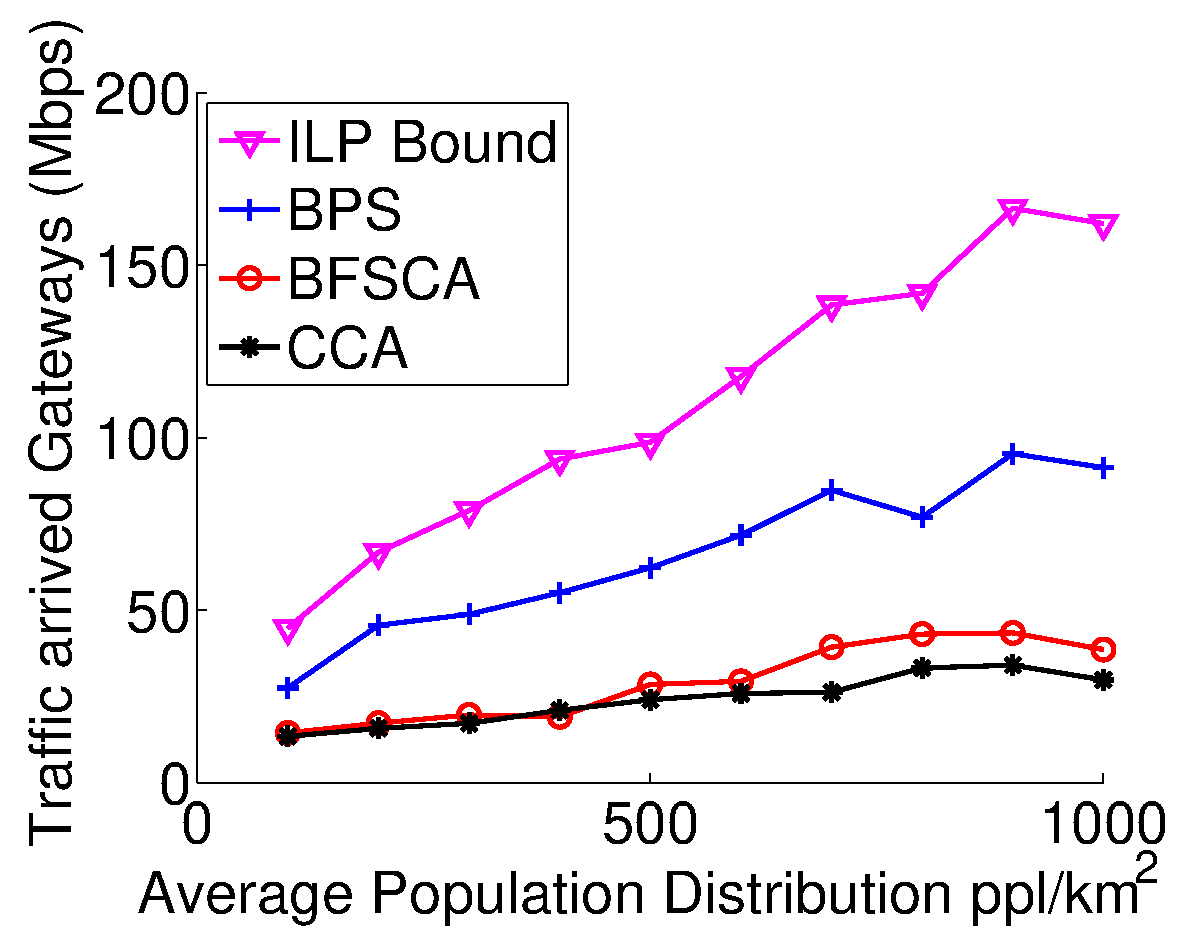
\includegraphics[width=74mm]{figures/maxtpt}
   \vspace{-0.1in}
   \caption{Varying maximum offered load for a 30-node regular-grid mesh topology.}                                                                               
   \label{fig:maxtpt}
   %\vspace{-0.0in}
   \end{figure}
   BPS performs better than the other 3 algorithms since during the channel assignment process, it is already optimize the paths from further nodes to gateways make it possible to ship data from these nodes. But as the max offer load increase, all the channel assignment suffer the bottle neck of link capacity.



   To evaluate the performance in different size of network, we fix the max offer load of each node as $5MB/s$ and vary the number of nodes in the regular grid network. The performance of the algorithms are shown in ~\ref{fig:varysize}. 
   \begin{figure}
   %\vspace{-0.0in}
   \centering
   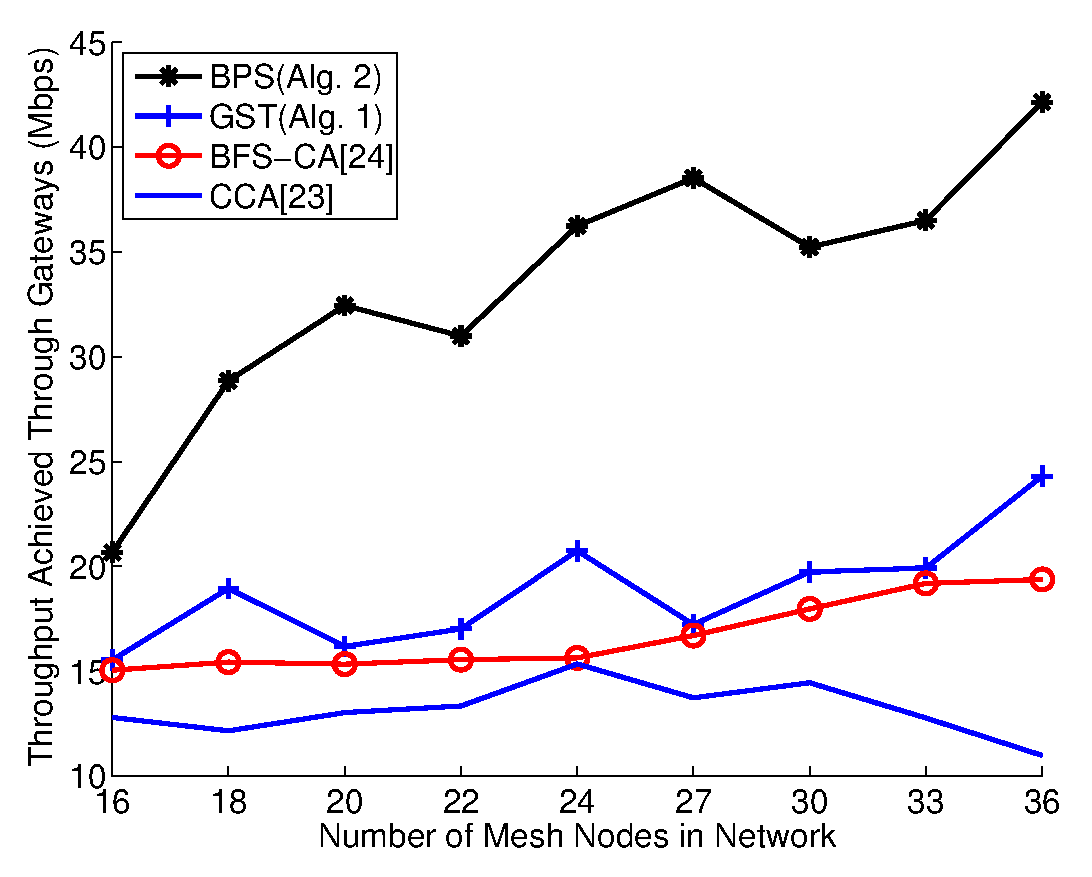
\includegraphics[width=74mm]{figures/varysize}
   \vspace{-0.1in}
   \caption{Uniform offered load per mesh node of 4 Mbps.}                                                                 
   \label{fig:varysize}
   %\vspace{-0.0in}
   \end{figure}

   As the number of mesh node increase, CCA lose the ability to handle large size of network. The dips of the curves are resulting from the evaluation setup. We randonly deploy the gateways and offer load of each mesh node, that brings the decrease in achieving throughput when the number of mesh node increase. BSP and GST performs better than other previous algorithms in different size of network.


   Our simulation also shows the importance of channel selection of multiband. ~\ref{tab:2channelcombination} shows when 2 radios could be used, the better combination would be a higher frequency and a lower frequency. 
   Two low frequency channel, as in ~\ref{tab:2channelcombination}, will bring more interference to the network.
   In this scenario, the performance is even worse than use WiFi channel only. The reason two low frequency channels has better than WiFi only due to the channel assignment fails to connect all mesh node to the gateways make there exist some offer load can not be shipped to gateways.
   So a smart way to choose channels is to select a set of channels in different band rather than select channels has the same propagation characteristics.

   % Use table to replace the hint graph


   \begin{table*}[t] 
   \centering % centering table 
   \begin{tabular}{|l|c|c|c|c|c|c|c|c|c|c|c|} % creating 12 columns 
   \hline %\hline % inserting double-line 
   Bands/     & WiFi    & WS      & WS \& & WS \& &  WS \& & WS \& & WS \&      &  WS \&      & Multi-WS \& & Multi-WS \& & Multi-WS \& \\% [0.5ex]
   Algorithms & Only    & Only    & WiFi  & WiFi  &  WiFi  & WiFi  & Multi-WiFi &  Multi-WiFi & WiFi        & WiFi        & Multi-WiFi  \\
	   \hline % inserts single-line 
	   % Entering 1st row 
	   WS (MHz)   &							    & 450,900 & 450 &  900  &  450   & 900		 & 450    & 900      & 450,900     & 450,900     & 450,900     \\
		   \hline
		   WiFi (GHz) & 2.4,5.8 &								  & 2.4 &  2.4  &  5.8   & 5.8		 & 2.4,5.8& 2.4,5.8	 & 2.4		   & 5.8         & 2.4,5.8     \\ % [0.5ex]
		   \hline
		   \hline % inserts single-line 
		   CCA~\cite{draves2004routing}			    & 3.1   &  7.3  & 8.2    &8.1    &8.3		 &7.8     &   8.7    &   9.3&     9.0             &         11.9     &   14.4          \\
			   \hline % inserts single-line                                                                                                       
			   BFSCA~\cite{ramachandran2006interference}  & 8.9   &  6.2  & 7.9    & 9.0   & 13.6 	 & 13.8   &  14.9    &   13.8&      14.9           &      14.3       &       18.6      \\ 
			   \hline % inserts single-line                                                                                                      
			   GST (Alg. 1)								& 11.6  &   6.6 & 9.3    &   15.1&   15.8	 &  14.4  &   16.6   &    14.1  &   18.8            &  15.0           &    25.1         \\
				   \hline % inserts single-line                                                                                                     
				   BPS (Alg. 2)								& 22.2  & 18.2  &  28.4  & 25.0  & 30.9 	 & 25.8   &   32.00  &  33.5       &     34.5            &      30.9       &       35.2      \\ 
				   \hline % inserts single-line 
				   \end{tabular} 
				   \label{tab:2channelcombination} 
				   \caption{Throughput achieved through Gateway nodes (Mbps) for various combinations of WiFi and White Space (WS) mesh topologies (Offered Load = 4 Mbps, Network Size = 30 mesh nodes).} % title name of the table 
				   \vspace{-0.1in}
				   \end{table*} 

				   %
				   %				   \begin{table}[h] 
				   %				   \centering % centering table 
				   %				   \begin{tabular}{|p{1.2cm}| p{1.2cm} | p{0.9cm} | p{1.2cm} |p{1.1cm}|p{1.2cm}|} % creating 10 columns 
				   %				   \hline %\hline % inserting double-line 
				   %				   \multirow{2}{*}{Type} & \multirow{2}{*}{Bands} & \multicolumn{4}{c|}{Algorithms}   \\% [0.5ex]
				   %				   \cline{3-6}
				   %				   %  \hline
				   %				   & & CCA[23] & BFSCA[24] & GST(Alg.1) & BPS(Alg.2) \\ [2ex]
				   %				   % \\ [0.5ex] 
				   %				   \hline % inserts single-line 
				   %				   WiFi Only & $2.4+5G$ & 3.0912 & 8.9460 & 11.5934 & 22.2179 \\ [2ex]
				   %				   \hline % inserts single-line 
				   %				   WS Only & $450+900M$ & 7.3428 & 6.2115 & 6.5567 & 18.1946 \\[2ex]
				   %				   \hline % inserts single-line 
				   %				   \multirow{4}{*}{\begin{minipage}{0.5in}WiFi +WS\end{minipage}} & 2.4G+450M & 8.2168 & 7.9206 & 9.2521 & 28.4069 \\[2ex]
				   %				   \cline{2-6} % inserts single-line 
				   %				   & $2.4G+900M$ & 8.1321 & 8.978 & 15.0802 & 24.985 \\[2ex]
				   %				   \cline{2-6} % inserts single-line 
				   %				   & $5G+450M$ & 8.3416 & 13.5729 & 15.8455 & 30.9351 \\[2ex]
				   %				   \cline{2-6} % inserts single-line 
				   %				   &$ 5G+900M$ & 7.8412 & 13.8290  & 14.4036 & 25.8345 \\[2ex]
				   %				   \hline % inserts single-line 
				   %				   WiFi+ Multi-WS &$2.4G+450M+900M$  & 8.9788 & 14.9167 & 18.7859& 34.5374 \\[2ex]
				   %				   \hline % inserts single-line 
				   %				   Multi-WiFi+WS & $2.4G+5G+450M$ & 8.6892 &14.9167 &16.6344 &31.9532  \\[2ex]
				   %				   \hline % inserts single-line 
				   %				   Multi-WiFi+Multi-WS & $2.4G+5G+450M+900M$ &14.3703  & 18.6406 &25.0988 & 53.1671 \\[2ex]
				   %				   \hline % inserts single-line 
				   %				   \end{tabular} 
				   %				   \label{tab:2channelcombination} 
				   %				   \caption{Various combinations of WiFi and White Space mesh topologies (offered load = 5Mbps, network size = 30).} % title name of the table 
				   %				   \vspace{-0.1in}
				   %				   \end{table} 
				   %
				   %
				   %\begin{table*}
				   %				   \centering % centering table 
				   %				   \begin{tabular}{|p{1.3cm}| p{1.3cm} | p{1.3cm} | p{1.3cm} |p{1.3cm}|p{1.3cm}|} % creating 10 columns 
				   %				   \hline %\hline % inserting double-line 
				   %				   \multirow{2}{*}{Type} & \multirow{2}{*}{Bands} & \multicolumn{4}{c}{Algorithms}   \\% [0.5ex]
				   %				   \cline{3-6}
				   %				   %  \hline
				   %				   & & CCA[23] & BFSCA[24] & GST(Alg.1) & BPS(Alg.2) \\ [2ex]
				   %				   % \\ [0.5ex] 
				   %\end{table}
				   %

The number of radio equipped on a node in mesh network also abstract ISP attention. 
The result shows in ~\ref{fig:varyradios}, BPS has the best performance over other algorithms. 
Increasing radios do improve the performance of network. 
As more radios equipped in the network, the benefit would be decrease in most scenario. 
There is a tradeoff between performance of more radios and cost increading.
In one radio scenario, BPS outperforms CCA, but fails in completion of BFS-CA and GST.
But in multi-radio scenarios, our BPS always outperforms the other methods.


\begin{figure}
%\vspace{-0.0in}
\centering
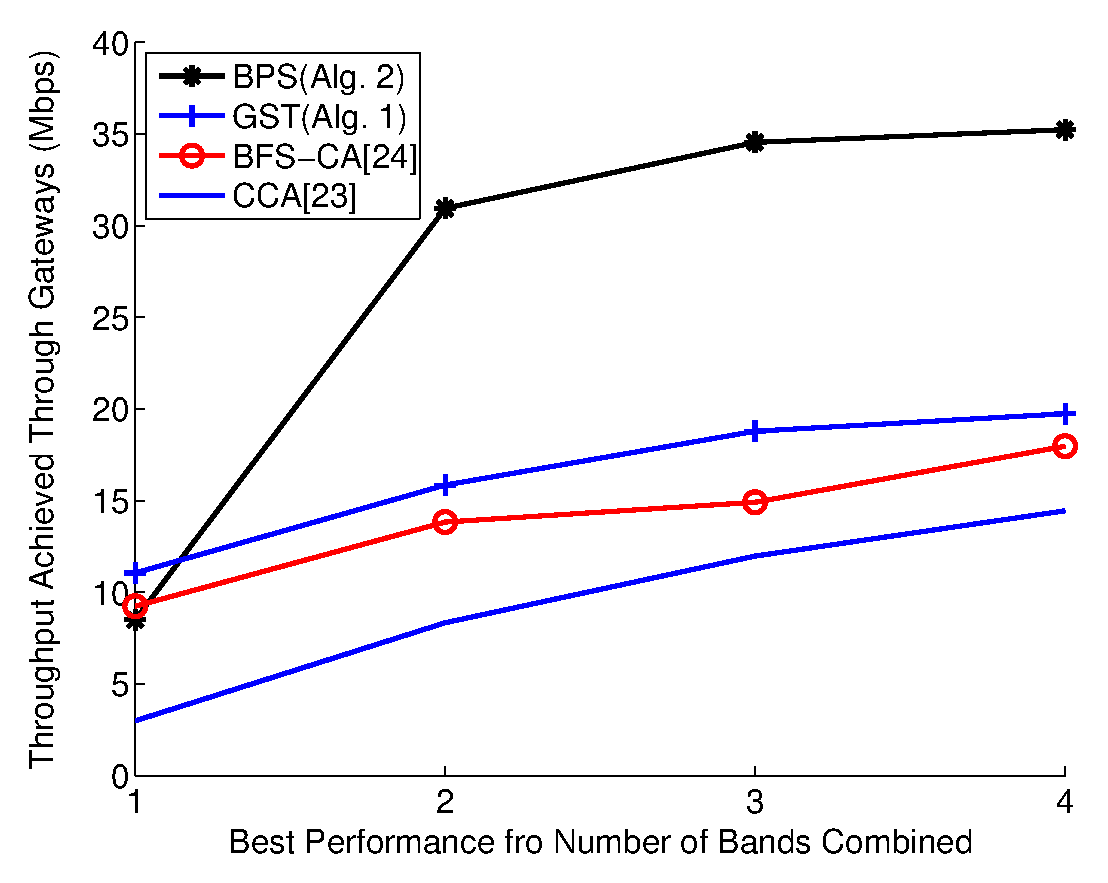
\includegraphics[width=74mm]{figures/varyradios}
\vspace{-0.1in}
\caption{Varying radios in 30-node regular-grid of 4 Mbps.}                                                                               
\label{fig:varyradios}
%\vspace{-0.0in}
\end{figure}





\begin{figure}
%\vspace{-0.0in}
\centering
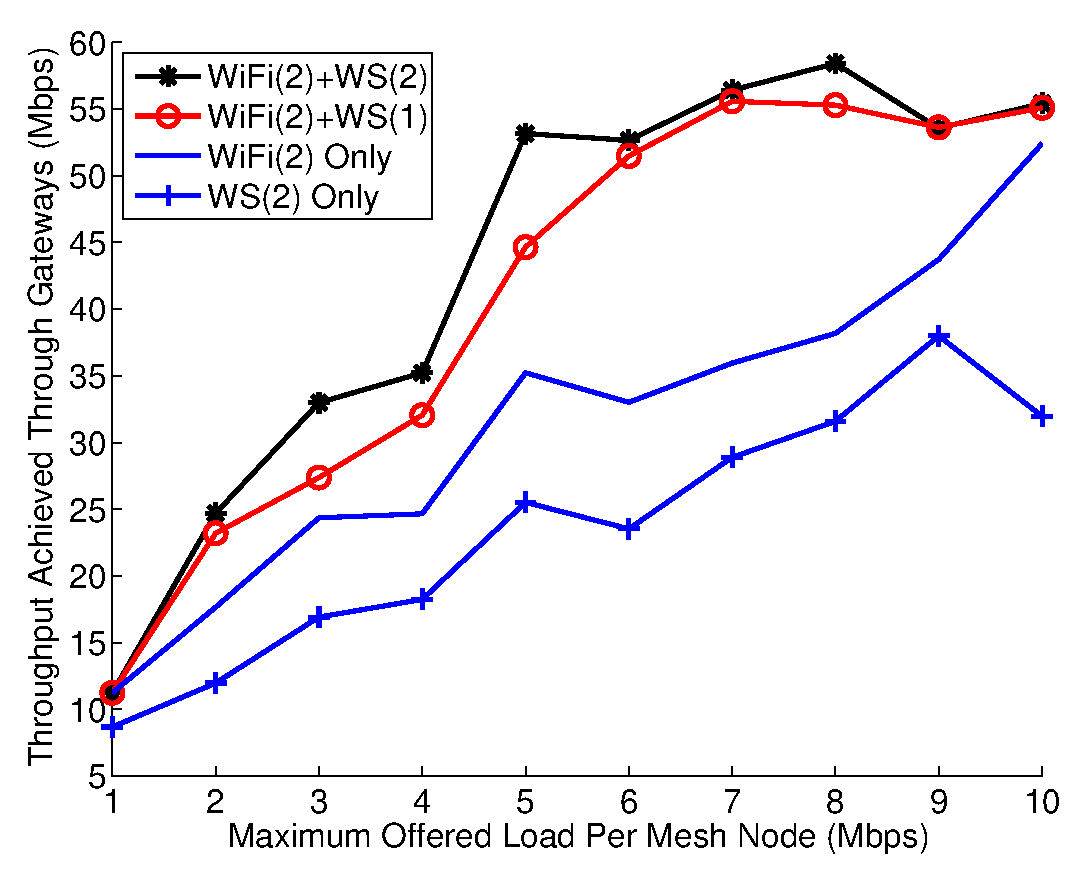
\includegraphics[width=74mm]{figures/wifiws}
\vspace{-0.1in}
\caption{WiFi White Space Combination Performance}                                                                               
\label{fig:wifiws}
%\vspace{-0.0in}
\end{figure}

